\documentclass[a4paper,12pt]{article}
\usepackage{amsmath}
\usepackage{xcolor}
\usepackage{tikz}
\usepackage{graphicx}
\usetikzlibrary{shapes.geometric, arrows}

\title{Soal Cerita Kalkulator Luas Bangun Datar}
\author{}
\date{}

\begin{document}
\maketitle

\section*{Soal Cerita Kalkulator Luas Bangun Datar}

Dalam aplikasi ini, kita akan menghitung luas bangun datar berdasarkan pilihan pengguna. Berikut adalah beberapa kasus yang ingin dihitung luasnya:

\subsection*{1. Menghitung Luas Persegi}
Sebuah persegi memiliki panjang sisi 4 meter. Hitunglah luas persegi tersebut!

\begin{center}
\begin{tikzpicture}
    \draw[thick] (0,0) rectangle (4,4);
    \node at (2, -0.5) {4 m};
    \node at (-0.5, 2) {4 m};
    \node at (2, 2) {Persegi};
\end{tikzpicture}
\end{center}

Rumus luas persegi adalah:
\[
L = s^2
\]
di mana \(s\) adalah panjang sisi.

\subsection*{2. Menghitung Luas Lingkaran}
Diberikan sebuah lingkaran dengan jari-jari 7 cm. Hitunglah luas lingkaran tersebut!

\begin{center}
\begin{tikzpicture}
    \draw[thick] (0,0) circle (3.5);
    \node at (0, -4) {7 cm};
    \node at (0, 0) {Lingkaran};
\end{tikzpicture}
\end{center}

Rumus luas lingkaran adalah:
\[
L = \pi r^2
\]
di mana \(r\) adalah panjang jari-jari lingkaran.

\subsection*{3. Menghitung Luas Segitiga}
Sebuah segitiga memiliki panjang alas 6 cm dan tinggi 8 cm. Hitunglah luas segitiga tersebut!

\begin{center}
\begin{tikzpicture}
    \draw[thick] (0,0) -- (6,0) -- (3,8) -- cycle;
    \node at (3, -0.5) {6 cm};
    \node at (-0.5, 4) {8 cm};
    \node at (3, 4) {Segitiga};
\end{tikzpicture}
\end{center}

Rumus luas segitiga adalah:
\[
L = \frac{1}{2} \times a \times t
\]
di mana \(a\) adalah panjang alas dan \(t\) adalah tinggi segitiga.

\subsection*{Tugas Anda}
Buatlah aplikasi kalkulator untuk menghitung luas bangun datar di atas! Aplikasi tersebut harus dapat menghitung luas persegi, lingkaran, dan segitiga berdasarkan input dari pengguna. Untuk setiap bangun datar, tampilkan hasilnya sesuai dengan rumus yang relevan.

\section*{Petunjuk}
\begin{itemize}
    \item Pilih jenis bangun datar yang ingin dihitung luasnya (persegi, lingkaran, atau segitiga).
    \item Masukkan panjang sisi (untuk persegi), jari-jari (untuk lingkaran), atau alas dan tinggi (untuk segitiga).
    \item Aplikasi akan menghitung dan menampilkan hasil luas berdasarkan rumus yang sesuai.
\end{itemize}

\newpage

\section*{Flowchart Kalkulator Luas Bangun Datar}

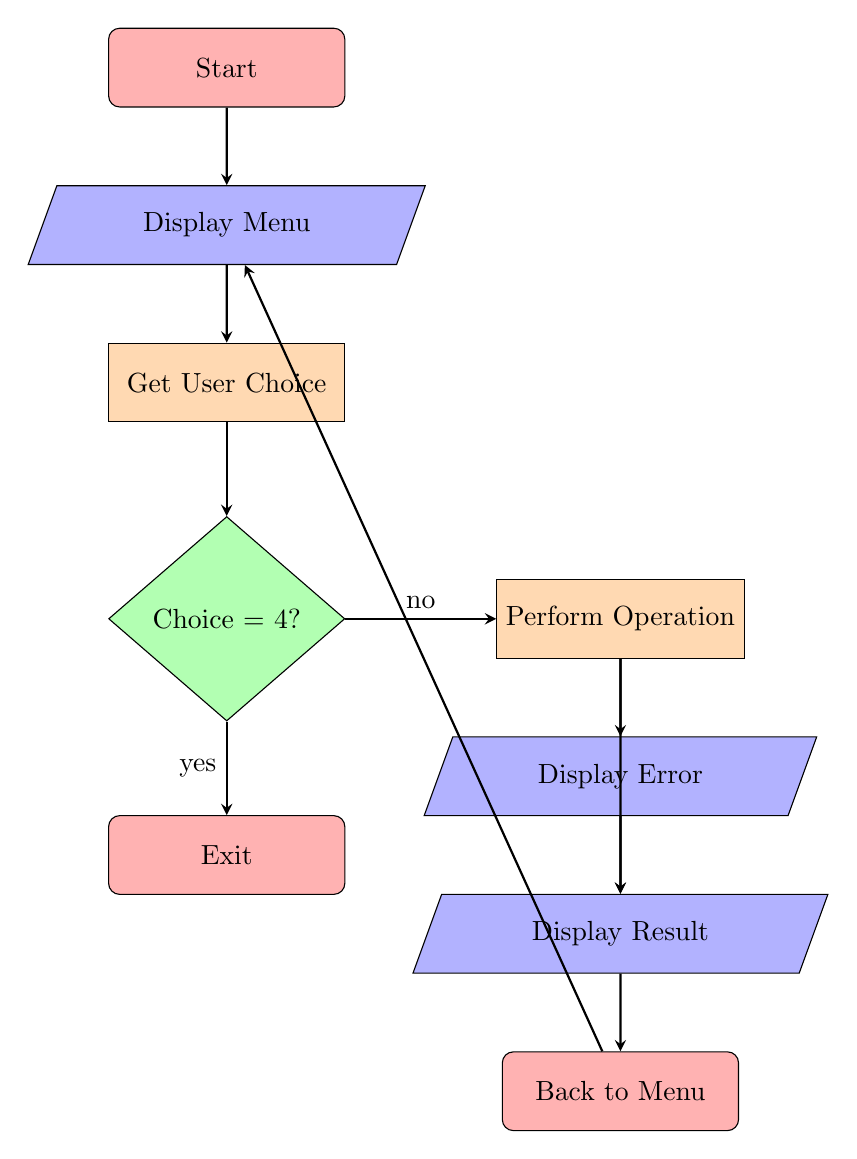
\begin{tikzpicture}[node distance=2cm]

\tikzstyle{startstop} = [rectangle, rounded corners, minimum width=3cm, minimum height=1cm, text centered, draw=black, fill=red!30]
\tikzstyle{io} = [trapezium, trapezium left angle=70, trapezium right angle=110, minimum width=3cm, minimum height=1cm, text centered, draw=black, fill=blue!30]
\tikzstyle{process} = [rectangle, minimum width=3cm, minimum height=1cm, text centered, draw=black, fill=orange!30]
\tikzstyle{decision} = [diamond, minimum width=3cm, minimum height=1cm, text centered, draw=black, fill=green!30]
\tikzstyle{arrow} = [thick,->,>=stealth]

% Nodes
\node (start) [startstop] {Start};
\node (menu) [io, below of=start] {Display Menu};
\node (choice) [process, below of=menu] {Get User Choice};
\node (checkchoice) [decision, below of=choice, yshift=-1cm] {Choice = 4?};
\node (exit) [startstop, below of=checkchoice, yshift=-1cm] {Exit};
\node (operation) [process, right of=checkchoice, xshift=3cm] {Perform Operation};
\node (error) [io, below of=operation] {Display Error};
\node (result) [io, below of=error] {Display Result};
\node (loop) [startstop, below of=result] {Back to Menu};

% Arrows
\draw [arrow] (start) -- (menu);
\draw [arrow] (menu) -- (choice);
\draw [arrow] (choice) -- (checkchoice);
\draw [arrow] (checkchoice) -- node[anchor=east] {yes} (exit);
\draw [arrow] (checkchoice) -- node[anchor=south] {no} (operation);
\draw [arrow] (operation) -- (result);
\draw [arrow] (result) -- (loop);
\draw [arrow] (loop) -- (menu);
\draw [arrow] (operation) -- (error);
\draw [arrow] (error) -- (result);

\end{tikzpicture}

\end{document}
